\section{Related Work}

\begin{figure*}[t]
  \centering
  \begin{subfigure}{.4\linewidth}
    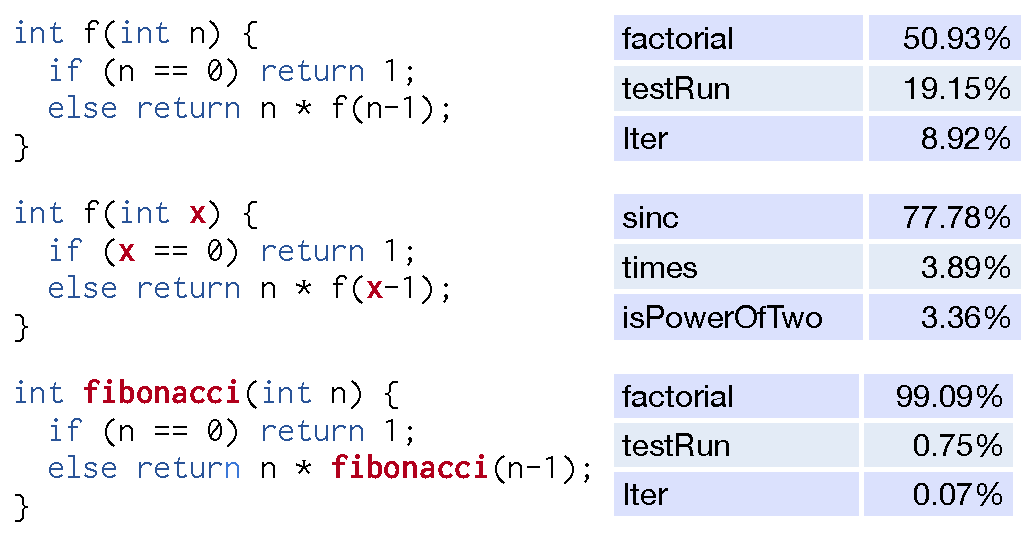
\includegraphics[width=\linewidth]{images/code2vec.pdf}
    \caption{code2vec is sensitive to naming over semantics. }
    \label{subfig:code2vec}
  \end{subfigure}
  \hfill
  \begin{subfigure}{.15\linewidth}
    \vspace{1.5em}
    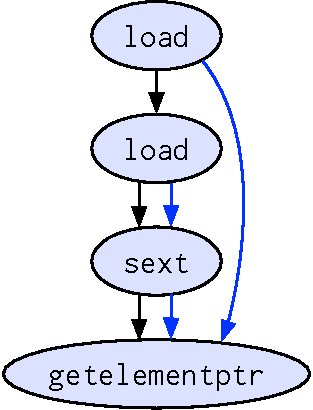
\includegraphics[width=.9\linewidth]{images/cdfg.pdf}
    \caption{CDFG omits operands.}
    \label{subfig:cdfg}
  \end{subfigure}
  \hfill
  \begin{subfigure}{.3\linewidth}
    \vspace{2em}
    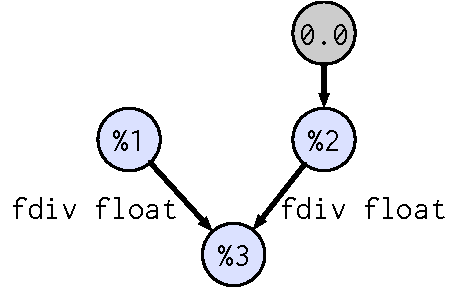
\includegraphics[width=.9\linewidth]{images/inst2vec.pdf}
    \caption{XFG cannot distinguish non-commutative statements.}
    \label{subfig:inst2vec}
  \end{subfigure}
  \vspace{-.3em}
  \caption{%
    Limitations in state-of-the-art learnable code representations:
    code2vec~\citep{Alon2018a}, CDFG~\citep{Brauckmann2020}, and
    XFG~\citep{Ben-nun2018}.
    \vspace{-1em}
  }
\end{figure*}

Data flow analysis is a long established area of work firmly embedded in modern
compilers. Despite its central role, there has been limited work in learning
such analysis. \citet{Bielik2017a} use ASTs and code synthesis to learn
rule-sets for static analyses, some of which are dataflow-related. Our approach
does not require a program generator or a hand-crafted DSL for rules.
\citet{Shi2019} and \citet{wang2020blended} use dynamic information (e.g.,
register snapshots and traces) from instrumented binaries to embed an assembler
graph representation. We propose a static approach that does not need runtime
features. \citet{Si2018} use a graph embedding of an SSA form to generate
invariants. The lack of phi nodes and function call/return edges means that the
representation is not suitable for interprocedural analysis as it stands.
\citet{Kanade2019} explore a large-scale, context-dependent vector embedding.
This is done at a token level, however, and is unsuited for dataflow analysis.

Prior work on learning over programs employed methods from Natural Language
Processing that represented programs as a sequence of lexical
tokens~\citep{Allamanis2016d,Cummins2020}. However, source-level representations
are not suited for analyzing partially optimized compiler IRs as the input
source cannot be recovered. In program analysis it is critical to capture the
structured nature of programs~\citep{Raychev2015,Allamanis2017b,Alon2018c}.
Thus, syntactic (tree-based) as well as semantic (graph-based) representations
have been proposed~\citep{Allamanis2017a,Brauckmann2020}. \citet{Dam2018}
annotate nodes in Abstract Syntax Trees (ASTs) with type information and employ
Tree-Based LSTMs~\citep{Tai2015a} for program defect prediction. Both
\citet{Raychev2015} and \citet{Alon2018a,Alon2018c} use path-based abstractions
of the AST as program representations, while \citet{Allamanis2017b} augment ASTs
with a hand-crafted set of additional typed edges and use GGNNs~\citep{Li2015a}
to learn downstream tasks related to variable naming. Another line of research
considers modelling binary similarity via control-flow graphs (CFGs) with an
adaptation of GNNs called Graph Matching Networks~\citep{Li2019}.

The history of IR-based graph representations for optimization goes back
to~\citet{Ferrante1987}, who remove superfluous control-flow edges to ease
optimization with a compact graph representation. A more contemporary precursor
to our approach is the ConteXtual Flow Graph (XFG)~\citep{Ben-nun2018}, which
combines control-flow with data-flow relations in order to learn unsupervised
embeddings of LLVM-IR statements. XFGs omit information that is critical to
analysis including the notion of argument order, vertices for both variables and
constants, and all control-flow edges. \programl, in combining call-graphs (CG),
control-flow graphs, and data-flow graphs (DFG), offers an IR-level program
representation that is designed to be useful for a variety of purposes from
specific program analyses to downstream optimization tasks.
\citet{steiner2021value} propose a representation based on data flow graphs
where each node uses a hand crafted feature representation. The graphs are then
serialized and processed using LSTMs. Control and Data Flow Graphs
(CDFG)~\citep{Brauckmann2020} use graph vertices for statements and have
bi-directional edges for control and data dependencies. The CDFG uses only the
instruction opcode to represent a statement, omitting operands, variables, data
types, and constants. This prohibits the reasoning about variables and
expressions that are required for many data flow analyses, including 3 out of
the 5 benchmark tasks that we establish below. \citet{mendis2019compiler}
represent LLVM-IR using a graph that is specialized to a vectorization task.
They use unique edge types to differentiate the first five operand positions and
augment the graph structure with vectorization opportunities that they compute a
priori. Our approach is not specialized to a task, enabling such opportunities
learned (e.g., subexpression detection), and uses an embedding weighting to
differentiate edge positions without having to learn separate edge transfer
weights for each. Finally, an alternate approach is taken by
IR2Vec~\citep{KeerthyS2019}, an LLVM-IR-specific representation that elegantly
models part-of-statements as relations. However, in order to compute the values
of the embeddings, IR2Vec requires access to the type of data flow analyses that
our approach learns from data alone.
